\documentclass{beamer}
\usetheme{CambridgeUS}

\usepackage{tikz}
\usetikzlibrary{calc,positioning}

\title{Interest Rate Swap}
\author{Matteo Sani}
\begin{document}
	\begin{frame}[plain]
		\maketitle
	\end{frame}
	
	\AtBeginSection{
		\begin{frame}{Outline}
			\tableofcontents[currentsection]
		\end{frame}
	}

\begin{frame}{Interest Rate Swap}
	\begin{itemize}
		\item An \textcolor{red}{Interest Rate Swap} (IRS) is a contract that exchanges payments between two differently indexed "legs", starting from a future time instant. At every pre-specified instant $T_i$, the fixed leg pays the amount
		\begin{equation*}
			N\tau(T_{i-1}, T_i)K
		\end{equation*}
		while the variable leg pays the amount
		\begin{equation*}
			N\tau(T_{i-1}, T_i)L(T_{i-1}, T_i)
		\end{equation*}
		\item When the fixed leg is paid, the IRS is termed \textcolor{red}{Payer IRS}. If the opposite holds, we have a \textcolor{red}{Receiver IRS}.
		\item The discounted payoff of a Payer IRS can be expressed as:
		\begin{equation}
			\sum_{i=\alpha+1}^{\beta} D(t,T_i)N \underbrace{\tau_i}_{\tau(T_{i-1},T_i)}
			\left[L(T_{i-1},T_i)-K\right]
		\end{equation}	
	\end{itemize}
	
\end{frame}

\begin{frame}{IRS and FRA}
	\begin{itemize}
		\item We can view the last expression as a portfolio of FRAs though.
		\item Consider a Receiver IRS and express its payoff as a sum FRAs with Eq.~\ref{eq:fram_payoff_withF}
		\begin{equation}
			\begin{aligned}
				\text{RFS}&(t,T,\tau,N,K) =N\sum_{i=\alpha+1}^{\beta}\tau_i P(t,T_i)(K-F(t;T_{i-1},T_i))\\
				&=N\sum_{i=\alpha+1}^{\beta}\tau_i KP(t,T_i)-N\sum_{i=\alpha+1}^{\beta}(P(t,T_{i-1})-P(t,T_i)) \\
				&=N\sum_{i=\alpha+1}^{\beta}\tau_i KP(t,T_i)-NP(t,T_\alpha)+NP(t,T_\beta)
			\end{aligned}
		\end{equation}
	\end{itemize}
\end{frame}

\begin{frame}{Swap Rates as Break-even Rates}
	\begin{itemize}
		\item The fixed rate $K$ which makes the above expression null is called \textcolor{red}{forward swap rate}:
		\begin{equation}
			S_{\alpha,\beta}(0) = \frac{P(0, T_\alpha)-P(0,T_\beta)}{\sum_{i=\alpha+1}^{\beta}\tau_iP(0,T_i)}
		\end{equation}
		\item if $T_\alpha=0$ we have the \textcolor{red}{spot swap rate} (which is published on financial newspapers).
		\item The swap rate makes the contract fair at inception by definition.
	\end{itemize}
\end{frame}

\begin{frame}{Swap and FRA Rates}
	\begin{itemize}
		\item Clearly not all the FRAs in a swap with zero value have zero value (except for the degenerate case of flat yield curve): some of them will have positive NPV, some other negative; the only constraint being their sum is zero.
		\item In a \emph{payer swap} with an increasing yield curve the first FRAs will have negative value, the last positive. Still their NPV's sum is zero.
		\item If the market don't move so much the swap rate payer will have to pay a net interest differential in the first part of the contract life, and to receive net interest in the second.
		\item So the rate payer will have to fund the payments for the first part of the contract and to invest at his best the receipt during the second part. (This is a very hot topic nowadays; this feature is sometimes referred to as the funding profile of the contract).
	\end{itemize}
	\begin{tikzpicture}[remember picture,overlay]
		\node[xshift=5cm,yshift=-3.7cm] at (current page.center) {
\includegraphics[width=30px]{python_logo}};
	\end{tikzpicture}
\end{frame}

\begin{frame}{An Alternative Expression for the Swap Payoff}
	\begin{itemize}
		\item Consider a Payer IRS with $N=1$:
		\begin{equation*}
			\text{PFS} = P(t,T_\alpha)-P(t,T_\beta)-\sum_{i=\alpha+1}^{\beta}\tau_iKP(t,T_i)
		\end{equation*}
		\item By multiplying and dividing by
		\begin{equation}
			A = \sum_{i=\alpha+1}^{\beta}\tau_iP(t, T_i)
		\end{equation}
		we get...
	\end{itemize}
\end{frame}

\begin{frame}{An Alternative Expression for the Swap Payoff}
	\begin{equation*}
		\text{PFS}=\frac{A}{\sum_{i=\alpha+1}^{\beta}\tau_iP(t, T_i)}\left[P(t,T_\alpha)-P(t,T_\beta)-\sum_{i=\alpha+1}^{\beta}\tau_iKP(t,T_i)\right]
	\end{equation*}
	\begin{itemize}
		\item It follows
		\begin{equation}
			\text{PFS}=A (S_{\alpha,\beta}(t)-K)
		\end{equation}
		\item This expression will be useful when pricing swaptions.
	\end{itemize}
\end{frame}

\begin{frame}{Swaps and Bonds}
	\begin{itemize}
		\item Consider again a Payer Forward Swap
		\begin{equation*}
			\text{PFS}(t,T_\alpha,T_\beta,\tau,N,K)=N(P(t,T_\alpha)-P(t,T_\beta))-N\sum_{i=\alpha+1}^{\beta} K\tau_iP(t,T_i)
		\end{equation*}
		\item When $T_\alpha = t$, i.e. we take the particular case of spot trading (PFS becomes...PS). We thus get
		\begin{equation*}
			\begin{aligned}
				\text{PS}(t,T_\beta) &=N-\underbrace{NP(t,T_\beta)}_{\text{notional exch.}}-\underbrace{KN\sum_{i=\alpha+1}^{\beta} \tau_iP(t,T_i)}_{\text{coupons exch.}} \\
				&=N-\textbf{CBP}(t,T_\beta,K,N)
			\end{aligned}
		\end{equation*}
	\end{itemize}
\end{frame}

\begin{frame}{Fixed Rate Side}
	\begin{itemize}
		\item Last equation rearranged gives
		\begin{equation}
			\textbf{CBP}(t,T_\beta,K,N) = N - PS(t,T_\beta)
		\end{equation}
	\end{itemize}
	\begin{block}{Intepretation}
		The meaning is pretty straightforward: a fixed rate bond can be replicated using the NPV of a payer swap whose fixed leg coincides with the fixed leg of the bond. The floating leg represents the funding of the bond, i.e. the interests the issuer must pay to raise funds in the interbank market when his spread over the benchmark LIBOR rate is null.
	\end{block}
\end{frame}

\begin{frame}{Swap and Bond Switching}
	\begin{itemize}
		\item A swap can be considered as an exchange between two kinds of bond with the same notional reimbursed at maturity. In fact, the fixed leg of the swap can be viewed as a fixed coupon stream, while the variable can be considered a floating rate note coupon stream. 
		\item More formally, consider a coupon bond that pays the following cash flows
		\newline
		$\mathcal{C}=[c_{\alpha+1},\ldots,c_\beta]$	on the schedule
		$T = [T_{\alpha+1},\ldots,T_\beta]$ with 
		\begin{equation*}
			c_i = N\tau K,\quad i<\beta
		\end{equation*}
		and 
		\begin{equation*}
			c_\beta=N\tau K+N
		\end{equation*}
		\item The coupon bond price can be written as
		\begin{equation}
			\textbf{CBP}(t,\mathcal{C},T)=\sum_{i=\alpha+1}^{\beta}c_i P(t,T_i)
		\end{equation}
	\end{itemize}
\end{frame}

\begin{frame}{Floating Rate Note}
	\begin{itemize}
		\item Next consider a floating rate note that pays coupons at dates
		\begin{equation*}
			T_{\text{payment}} = [T_{\alpha+1},\ldots,T_\beta]
		\end{equation*}
		coupons calculated at the LIBOR rate fixed in the previous period
		\begin{equation*}
			T_{\text{fixing}} = [T_{\alpha},\ldots,T_{\beta - 1}]
		\end{equation*}.
		\item At maturity $T_\beta$ the notional is reimbursed as before.
		\item To value the price of this note we change sign to the RFS
		\begin{equation*}
			\text{RFS} = -N(P(t,T_\alpha)-P(t,T_\beta))+N\sum_{i=\alpha+1}^{\beta}K\tau_i P(t,T_i)
		\end{equation*}
	\end{itemize}
\end{frame}

\begin{frame}{Floating Rate Side}
	\begin{itemize}
		\item We impose $K=0$, i.e. no fixed rate payments are done, and finally we insert the present value of the notional at maturity $NP(0,T_\beta)$.
		\item Hence
		\begin{equation}
			-\text{RFS}(t,\tau,N,0) + NP(t,T_\beta) = NP(t,T_\alpha)
		\end{equation}
	\end{itemize}
	\begin{block}{Interpretation}
		The intuition behind this formula is again straightforward: if we set $T_\alpha =t$. At the date of the first reset, the bond price equals par. This result also holds for all the dates equal to the reset of the floating rates. 
	\end{block}
	This is an alternative proof that to avoid arbitrage opportunities, floating rate notes must trade at par.
	DA CAPIRE L'ULTIMA INTERPRETAZIONE
	%\item Provide an example of Italian government floating rate note. Did they trade at par in recent times ? Provide an explanation.
\end{frame}

\begin{frame}{Concepts behind the Formulas}
	Suppose that a generic Bank \emph{MyFavouriteBank} has the same credit risk of the corresponding average inter-bank entity. So, the spread over the LIBOR rate is 0. Suppose now the bank needs financing and it plans to issue coupon bonds. It has two alternatives:
	\begin{enumerate}
		\item borrow $N$ and pay floating interest at the rates
		\begin{equation*}
			L(T_{i-1},T_i)
		\end{equation*}
		\item borrow $N$ and pay fixed interest given by the coupon
		\begin{equation*}
			K = S_{\alpha,\beta}
		\end{equation*}	
	\end{enumerate}
\end{frame}

\begin{frame}{Concepts behind the Formulas}
	\begin{itemize}
		\item Clearly the overall cost to raise money must be the same at the beginning (fixed leg NPV equals floating leg NPV) and the bank will then opt for one of two alternatives depending on:
		\begin{enumerate}
			\item marketing considerations, i.e. which kind of bond people prefer;
			\item the interest rate risk it wants to have in a book.
		\end{enumerate} 
		\item Remember that a variable rate mortgage is perceived risky by the average individual as salary is more or less fixed, but for bank this is not the case because it is left unarmed by the rate rise. Indeed if rates go up
		\begin{itemize}
			\item the bank loses in the higher coupons it has to pay to the bond holders;
			\item the bank gains in the highest rates it charges on new loans at the same time.
		\end{itemize}
		\item This is the most basic example of asset liability matching.
		\item The same more or less holds for a rate decrease.%, but with some caveats.
	\end{itemize}
\end{frame}

\begin{frame}{Concepts behind the Formulas}
	\begin{itemize}
		\item Banks like floating rates exposure: as the liability value (the bond floating rate) resets with rates.
		\item Also floating interest rate debt often costs less than fixed-rate debt:
		\item  in compensation for lower fixed rate costs, borrowers must bear a higher interest rate risk (i.e. for bonds, risk of rates rising in the future). With inverted yield curve, the cost of debt may actually be higher than fixed-rate debt. However, this is the exception rather than the norm.
		\item  Floating rates are less expensive in the case of a long-term loan (e.g. 30-year mortgage), lenders require higher fixed rates for longer-term loans, due to bad accuracy in forecast economic conditions over such a long period of time.% There is a general assumption that interest rates will rise – or, increase – over time,
	\end{itemize}
\end{frame}

\begin{frame}{Concepts behind the Formulas}
	\begin{itemize}
		\item So why do not banks issue only floating rate notes ?
		\item Banks must issue fixed rate coupon bonds to attract customers (think of yourself or insurance companies) but then will hedge the liability  with an investment bank. In this way the final risk exposure will be at a variable rate as they like. 
		\item Swaps are both the hedging instrument and the pricing tool.% as formula above show.
	\end{itemize}
\end{frame}

\begin{frame}{Adding Credit Risk}
	\begin{itemize}
		\item When we make the real world enter the picture a typical bank will pay a spread over LIBOR representing credit risk (and other stuff, but leave this extra aside for the moment). 
		\item For the swap to be worth 0 at inception the fixed rate must clearly be higher then in the case of no spread. Hence a bank which has credit risk will have to pay
		\begin{enumerate}
			\item a higher coupon if it issues a bond with fixed coupon;
			\item a spread over the variable rate if it opts for a floating rate bond.
		\end{enumerate}
		\item Often, in the first case, it will swap the liability, i.e. the bank is liable towards the bond holders, to hedge the pure rate risk. 
		\item This lead us to the next topic, the asset swap and the asset swap spread.
	\end{itemize}
\end{frame}

\begin{frame}{Asset Swap}
	\begin{itemize}
		\item An \textcolor{red}{Asset Swap} (AS) can be defined as a \emph{synthetic floating-rate note}.
		\item In fact, the Asset Swap transforms a fixed rate in a floating rate, \emph{leaving the credit risk profile unchanged}.
		\item In the following we consider \textcolor{red}{Par Asset Swaps}. 
		\item The package is made of a position in a bond and another in a swap.
		\item In case of default, the Asset Swap buyer must pay the fixed leg and the principal in the swap but does not receive the coupon of the defaulted bond. 
	\end{itemize}
\end{frame}

\begin{frame}{Valuation of the Asset Swap}
	At valuation time $t$ the \emph{three} following facts are observed:
	\begin{itemize}
		\item the AS buyer in $t$ buys a generic \emph{risky} coupon bond $\overline{CB}(t,T,K,1)$ at the market price $\overline{CBP}$ from the AS seller;
		\item the AS seller pays/receives to/from the asset swap buyer the difference $\Delta = \overline{CBP}(t,T,K,N)-1$ in such a way that the net sum paid from the AS buyer is 1; hence if the bond trades above the par the difference $\Delta$ is paid to the AS buyer by the seller; conversely if the bond trades below par the difference $\Delta$ is paid to the AS seller by the buyer.
		\item A swap is then started between the two counter-parties such that the AS seller receives a fixed leg equal to the coupon stream of the bond and the AS buyer receives the floating leg given by the LIBOR rate plus a spread ($ASWS$).
	\end{itemize}
\end{frame}

\begin{frame}{Valuation of the Asset Swap}
	\begin{center}
		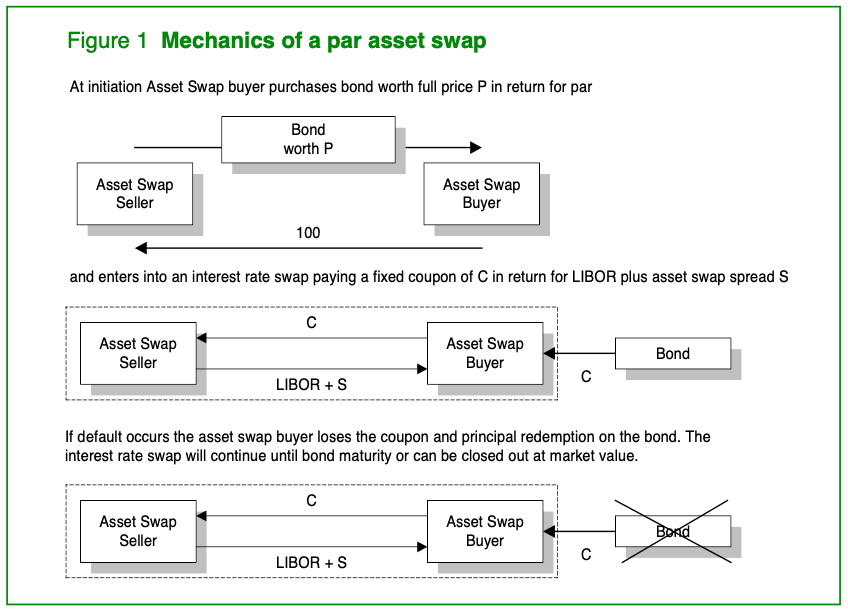
\includegraphics[width=0.8\linewidth]{asset_swap}
	\end{center}
\end{frame}

\begin{frame}{Valuation of the Asset Swap}
	\begin{itemize}
		\item From the perspective of the Asset Swap seller the value of the package is given by (we are considering spot trading so $T_\alpha = t = 0$)
		\begin{equation}
			\begin{aligned}
				1&-\overline{CBP}+K\sum_{i=\alpha+1}^{\beta}\tau_i P(0,T_i) \\
				&-\sum_{i=\alpha+1}^{\beta}\tau_i P(0,T_i)(L(T_{i-1},T_i)+ASWS)=0
			\end{aligned}
			\label{eq:asset_swap_value}
		\end{equation}
	\end{itemize}
\end{frame}

\begin{frame}{Valuation of the Asset Swap}
	\begin{itemize}
		\item We can replace the future rate with the forward rates, and after the substitution of $L$ with $F$ we can write
		\begin{equation}
			1 = \sum_{i=\alpha+1}^{\beta}\tau_i P(0,T_i)F(t,T_{i-1},T_i)+P(0,T_\beta)
		\end{equation}
		\item Hence 
		\begin{equation}
			1 - P(0,T_\beta) = \sum_{i=\alpha+1}^{\beta}\tau_i P(0,T_i)F(t,T_{i-1},T_i)
		\end{equation}
		\item Substitute into Eq~\ref{eq:asset_swap_value} to get
		\begin{equation}
			\begin{aligned}
				1&-\overline{CBP}+K\sum_{i=\alpha+1}^{\beta}\tau_i P(0,T_i) -(1-P(0,T_\beta)) \\
				&+ \sum_{i=\alpha+1}^{\beta}\tau_i P(0,T_i)ASWS=0
			\end{aligned}
		\end{equation}
	\end{itemize}
\end{frame}

\begin{frame}{Valuation of the Asset Swap}
	\begin{itemize}
		\item Canceling out the 1s
		\begin{equation}
			\begin{aligned}
				&-\overline{CBP}+K\sum_{i=\alpha+1}^{\beta}\tau_i P(0,T_i) +P(0,T_\beta) \\
				& + \sum_{i=\alpha+1}^{\beta}\tau_i P(0,T_i)ASWS=0
			\end{aligned}
		\end{equation}
		\item Finally we know that
		\begin{equation}
			K\sum_{i=\alpha+1}^{\beta}\tau_i P(0,T_i) + P(0,T_\beta)
		\end{equation}
		represents the price of coupons and principal of a bond priced off the LIBOR curve which we have assumed risk-free. We can denote it by $CBP$.
	\end{itemize}
\end{frame}

\begin{frame}{Asset Swap Spread}
	Solving for $ASWS$ we arrive at the final expression
	\begin{equation}
		ASWS = \frac{CBP-\overline{CBP}}{\sum_{i=\alpha+1}^{\beta}\tau_iP(0,T_i)}
	\end{equation}
	\href{https://colab.research.google.com/drive/1RrfmcrdqT4twtKr9HaDt4czR-HGSjivb?usp=share_link}{
		\begin{tikzpicture}[remember picture,overlay]
			\node[xshift=5cm,yshift=-3.7cm] at (current page.center) {
\includegraphics[width=30px]{python_logo}};
	\end{tikzpicture}}
\end{frame}

\begin{frame}{Asset Swap: Credit Considerations}
	\begin{itemize}
		\item As we have seen, in an Asset Swap the buyer takes on the credit risk of the bond. She is exposed to the loss of the coupons and redemption on the bond, i.e. the difference between the bond price and recovery value.
		%If the bond defaults, the asset swap buyer has to continue paying on the swap — which can no longer be funded with the coupon from the bond — or the swap can be closed out at market value. The asset swap buyer also loses the par redemption of the bond, receiving whatever recovery rate the bond issuer pays. 
		\item As a result the buyer has a default contingent exposure to the mark-to-market on the swap and to the redemption on the asset.  
		\item In economic terms the purpose of the Asset Swap Spread is to compensate the Asset Swap buyer for taking these risks.
		\item Since the $ASWS$ is quoted as a spread to LIBOR, for assets of better credit quality than AA-rated banks it may be negative.
	\end{itemize}
\end{frame}

\begin{frame}{Swap Delta Measures}
	\begin{itemize}
		\item \textbf{Basis Point Value:} the variation (in EUR) of the swap $NPV$ when the fixed rate is shifted by a basis point. It is equal to the present value of a one basis point rent, whose payments are scheduled according to the fixed leg of the swap:
		\begin{equation}
			BPV(t,T_\beta) = 0.01\%\sum_{i=\alpha+1}^{\beta}\tau_iP(0,T_i)
		\end{equation}
		\item \textbf{Market Rate Sensitivity:} it is given by the sum of the swap $NPV$ variations obtained by shifting one by one by a basis point the input market instruments of the yield curve used in the bootstrapping. In a standard plain vanilla swap is very close but does not coincide with the Basis Point Value. (Why ? Convexity is the answer.)
		\item \textbf{Modified Duration:} it is the relative variation of a bond price given the variation of the reference rate.
	\end{itemize}
	\href{shorturl.at/fBCK6}{
		\begin{tikzpicture}[remember picture,overlay]
			\node[xshift=5cm,yshift=-3.7cm] at (current page.center) {
\includegraphics[width=30px]{python_logo}
				shorturl.at/fBCK6};
		\end{tikzpicture}
	}
\end{frame}

\begin{frame}{Considerations}
	\begin{itemize}
		\item The mark to market value of the swap is a \emph{convex} function of the rates just in the same way a bond is a convex function of the yield.
		\item This is the reason why $BPV$ and sensitivity are not exactly the same number.
		\item Suppose for instance that we are short on a five year swap and to receive $4y$. If the rates go higher we lose money, but the rate of variation of the MTM decreases with the increases of rates. If rates decrease, the MTM increases, and the rate of variation of the MTM increase with the further increase with the further decrease of rates.
	\end{itemize}
\end{frame}

\begin{frame}{Considerations}
	\begin{itemize}
		\item Higher rates affect the $NPV$ in two ways: via the discounting and via the forecasting. If the rates go higher the present value of both legs is lower, but rhe forecasted value of the floating leg is higher: forward rates are higher.
		\item The total sensitivity is spread a bit along the curve even for bullet swaps also because of numerical factors.
		\item The way the curve is bootstrapped interferes with the calculation of the delta also for bullet swaps especially in the front end because the curve is bootstrapped uses different instruments.
	\end{itemize}
\end{frame}

\begin{frame}{Trading and Hedging Swaps}
	\begin{itemize}
		\item With a swap you can have a clear picture of the market. For example if you pay the 5Y, you make money if rates go higher, los money if they go lower.
		\item With two swaps you can bet on the \emph{slope} of the interest rate curve.
		\item If you bet on steepening of the 30y-10y slope, you pay the 10-30; if you bet on flattening on the same portion of the yield curve you receive the 10-30.
		\item Think of the economic determinants of the Steepening and flattening. Take the 30y-2y spread.
		\item With swaps you can bet on the \emph{bund basis}: this quantity is linked to the evolution of credit and liquidity in the interbank and Government bond markets.
	\end{itemize}
\end{frame}






\end{document}
